\documentclass[12pt]{article}
\usepackage{amsmath,amssymb,amsthm,graphicx}
\usepackage[utf8]{inputenc}
\usepackage{xcolor}
\usepackage{tikz}
\usepackage{pgfplots}
\pgfplotsset{width=10.5cm,compat=1.9}

\begin{document}

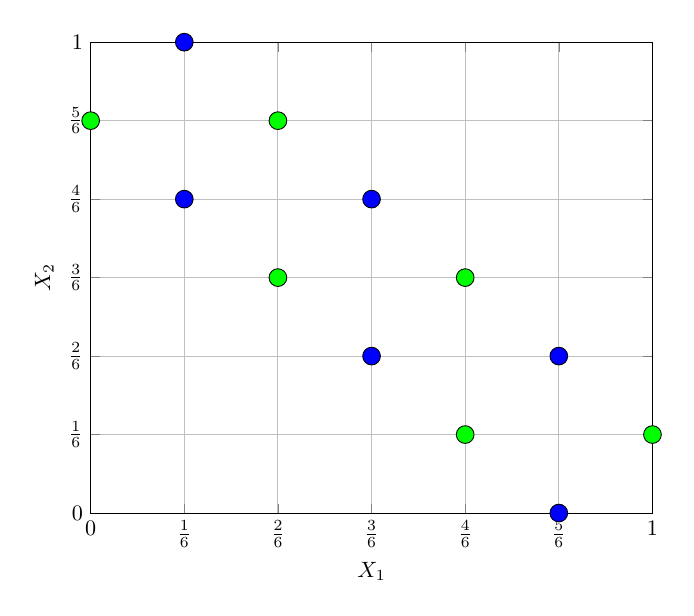
\begin{tikzpicture}[scale = 0.8]
  \begin{axis}[
    xlabel={$X_{1}$},
    ylabel={$X_{2}$},
    xmin=0,
    xmax=1,
    ymin=0,
    ymax=1,
    xtick={0,1/6, 2/6, 3/6, 4/6, 5/6, 6/6},
    xticklabels = {$0$,$\frac16$, $\frac26$, $\frac36$, $\frac46$, $\frac56$, $1$},
    xmajorgrids=true,
    ytick={0,1/6, 2/6, 3/6, 4/6, 5/6, 6/6},
    yticklabels = {$0$,$\frac16$, $\frac26$, $\frac36$, $\frac46$, $\frac56$, $1$},
    ymajorgrids=true,
    legend pos=south west,
  ]
  \addplot[only marks, color=black, ,mark=*,mark options={scale=2, fill=blue}] coordinates {(5/6, 0) (5/6, 1/3) (5/6-1/3, 1/3) (5/6-1/3, 2/3) (5/6-2/3, 2/3) (5/6 - 2/3, 1)};
  \addplot[only marks, color=black, ,mark=*,mark options={scale=2, fill=green}] coordinates {(0, 5/6) (1/3, 5/6) (1/3, 5/6-1/3) (2/3, 5/6-1/3) (2/3, 5/6-2/3) (1, 5/6 - 2/3) };
  \end{axis}
\end{tikzpicture}

\end{document}